\section{Loss Weights}\label{app:weights}

Table~\ref{tab:weights} lists the 13 loss terms and their weights. The weights were set by hand during development, using the training and validation splits only, and were not tuned by a search. Ablation A2 (Section~\ref{sec:ablations}) removes the two non-standard terms; the others are standard box, keypoint, heatmap and focal losses.

\begin{table}[h]
  \caption{Loss terms, their supervision, and weights.}
  \label{tab:weights}
  \footnotesize
  \begin{tabular}{llll}
    \toprule
    Term & Loss & Supervision & Weight \\
    \midrule
    Hand box & 1 $-$ CIoU & hand box & 0.10 \\
    Fingertip & Wing ($w{=}0.5$, $\epsilon{=}0.1$) & fingertip & 0.18 \\
    Direction & 1 $-$ cosine & fingertip $\to$ target centre & 0.03 \\
    Target box & 1 $-$ SIoU & target box & 0.45 \\
    Target box, auxiliary & 1 $-$ IoU & target box & 0.10 \\
    Hand gate & focal BCE, positives $\times3$ & $H$ & 0.08 \\
    Pointing gate & focal BCE, positives $\times2$ & $P$ (hand images) & 0.10 \\
    Target gate & focal BCE, positives $\times2$ & $T$ (pointing images) & 0.06 \\
    Ray alignment & distance to ray $+$ 0.5 $\cdot$ behind & none (predictions only) & 0.08 \\
    Hand axis & hinge outside a $60^\circ$ cone & none (predictions only) & 0.02 \\
    Hand heatmap & penalty-reduced focal, ownership-weighted & hand centre & 0.10 \\
    Fingertip heatmap & penalty-reduced focal & fingertip & 0.10 \\
    Target heatmap & penalty-reduced focal & target centre & 0.10 \\
    \bottomrule
  \end{tabular}
\end{table}

\section{Augmentation Parameters}\label{app:aug}

\begin{table}[h]
  \caption{Training-time augmentation, applied on the fly; each training image is seen once per epoch as a new random variant. Validation and test images are only resized and normalised.}
  \label{tab:aug}
  \footnotesize
  \begin{tabular}{lp{0.62\linewidth}}
    \toprule
    Step & Setting \\
    \midrule
    Distractor hands & 1--2 hands with probability 0.5 (hand images) or 0.3 (no-hand images); scale 0.45--1.0; rotation by 90/180/270$^\circ$ and optional mirror with probability 0.7; centre in the top 65\% of the frame; overlap with the wearer's hand and the target below 15\%; feathered alpha (12\% of the crop size); colour jitter; 30\% self-paste; pool of 512 donor crops, half from pointing hands \\
    Decoy patch & unlabelled non-hand patch from a no-hand image, with probability 0.15 \\
    Horizontal flip & 0.5 \\
    Shift / scale / rotate & ${\pm}5\%$ / ${\pm}10\%$ / ${\pm}15^\circ$, probability 0.4 \\
    Perspective & scale 0.02--0.05, probability 0.2 \\
    Brightness / contrast & ${\pm}20\%$, probability 0.5 \\
    Gaussian blur & kernel 3--5, probability 0.2 \\
    Mixup & within the same scene, $\lambda\sim\mathrm{Beta}(0.2,0.2)$ folded to ${\geq}0.5$, label of the dominant image, every batch \\
    Anchor forcing & ground-truth anchors with probability 0.5 decaying to 0 over 20 epochs \\
    \bottomrule
  \end{tabular}
\end{table}

\section{Additional Results}\label{app:extra}

\paragraph{Backbone.} Table~\ref{tab:backbone} replaces the ShuffleNetV2 0.5$\times$ backbone with MobileNetV3-Small~\cite{howard2019mobilenetv3} or MobileNetV4-Conv-Small~\cite{qin2024mobilenetv4}, with the recipe otherwise unchanged. Neither changes P@0.5 significantly, while doubling or nearly tripling the parameters. Both lean towards better large-gap accuracy (+5.7 and +4.8 points, intervals across 0) and a lower fingertip error (3.5 against 3.9\,px). Both runs stopped earlier (best epoch 64, against 100), so their numbers may be slightly low.

\begin{table}[h]
  \caption{Backbone swap at 160\,px, main-run recipe otherwise unchanged (one seed each). Target metrics in \%; brackets: 95\% paired-bootstrap interval of the difference from ShuffleNetV2.}
  \label{tab:backbone}
  \footnotesize
  \setlength{\tabcolsep}{4pt}
  \begin{tabular}{lrrrrrr}
    \toprule
    Backbone & Params & FP16 & GFLOPs & P@0.5 & Large-gap P@0.5 & Fingertip \\
    \midrule
    ShuffleNetV2 0.5$\times$ (ours) & 0.72M & 1.6\,MB & 0.231 & 58.9 & 25.4 & 3.9\,px \\
    MobileNetV3-Small & 1.57M & 3.2\,MB & 0.255 & 58.1 [$-$2.7, +1.0] & 31.1 [$-$0.5, +12.0] & 3.5\,px \\
    MobileNetV4-Conv-Small & 1.99M & 4.1\,MB & 0.398 & 59.8 [$-$0.9, +2.8] & 30.1 [$-$1.0, +10.5] & 3.5\,px \\
    \bottomrule
  \end{tabular}
\end{table}

\paragraph{IoU success curves.} Figure~\ref{fig:curves} shows how the share of successful hand and target boxes falls with the IoU threshold.

\begin{figure}[h]
  \centering
  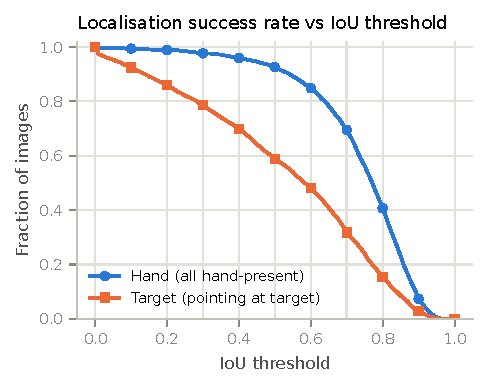
\includegraphics[width=0.48\linewidth]{figures/results/iou_success_rate}
  \caption{Share of test images whose hand or target box reaches each IoU threshold.}
  \Description{Two curves of success rate against IoU threshold; the hand curve stays above 0.9 up to IoU 0.5 and falls after 0.7, while the target curve falls steadily, reaching 0.59 at IoU 0.5 and 0.32 at 0.7.}
  \label{fig:curves}
\end{figure}

\paragraph{Failure types.} Figure~\ref{fig:qual} shows typical successes and one example of each failure type of Section~\ref{sec:qual}.

\begin{figure}[h]
  \centering
  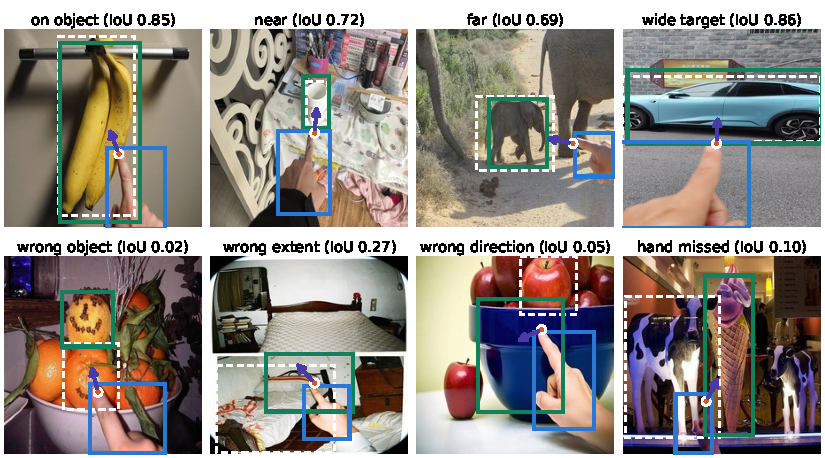
\includegraphics[width=\linewidth]{figures/qualitative}
  \caption{Successes (top) and failures (bottom) on EgoPoint test images: predicted hand (blue), fingertip and direction, and target (green); labelled target dashed. Bottom row, one example per failure type of Section~\ref{sec:qual}.}
  \Description{Eight egocentric images. Top row: correct target boxes for bananas touched by the finger, a cup near the finger, a young elephant far from the finger, and a car. Bottom row: a box on the wrong orange in a bowl of oranges, a box on part of a bed instead of the labelled bed, a box on a bowl while the label is an apple above it, and a frame where the hand gate missed the hand.}
  \label{fig:qual}
\end{figure}
